\documentclass[12pt]{article}

% Idioma e codificação
\usepackage[brazil]{babel}
\usepackage[utf8]{inputenc}
\usepackage[T1]{fontenc}

% Matemática e listas
\usepackage{amsmath, amssymb}
\usepackage{enumitem}
\usepackage{graphicx}
\usepackage{float}

% Layout e cores
\usepackage{geometry}
\usepackage{xcolor}

% Cores institucionais
\definecolor{maincolor}{RGB}{0,100,50}
\definecolor{forestgreen}{RGB}{0,100,50}

% Cabeçalho e rodapé
\usepackage{fancyhdr}

% Blocos
\usepackage[most]{tcolorbox}
\newtcolorbox{block}[1]{%
  colback=green!5,
  colframe=maincolor,
  coltitle=white,
  title=#1,
  fonttitle=\bfseries,
  boxrule=1.5pt,
  arc=3mm,
  left=6pt,
  right=6pt,
  top=6pt,
  bottom=6pt
}

% Margens
\geometry{margin=2.5cm}

% Fancyhdr
\pagestyle{fancy}
\fancyhf{}

\renewcommand{\headrulewidth}{2pt}
\renewcommand{\footrulewidth}{2pt}

\renewcommand{\headrule}{\hbox to\headwidth{%
  \color{forestgreen}\leaders\hrule height \headrulewidth\hfill}}

\renewcommand{\footrule}{\hbox to\headwidth{%
  \color{forestgreen}\leaders\hrule height \footrulewidth\hfill}}

% Altura do cabeçalho
\setlength{\headheight}{52pt}
\addtolength{\topmargin}{-20pt}

% Cabeçalho
\fancyhead[L]{%
  
\includegraphics[height=1.2cm]{Universidade_de_Rio_Verde.jpg}
}

\fancyhead[R]{%
  \raggedleft
  \textcolor{forestgreen}{%
    \small
    \textbf{Atividade Prática}\\
    Me.~Sergio Souza Novak\\
    \textit{Engenharia de Qualidade e Confiabilidade}
  }
}

% Rodapé
\fancyfoot[C]{\textcolor{forestgreen}{\thepage}}

% =========================
\begin{document}
% =========================

\vspace*{0.2cm}

\begin{center}
\Large \textbf{Atividade Prática — Análise de Logs de Servidor Web} \\

\normalsize Disciplina: Engenharia de Qualidade e Confiabilidade \\

\normalsize Tema: Análise de Logs e Desempenho de Sistemas
\end{center}

\vspace{0.5cm}

\section*{Objetivo}

\begin{block}{Objetivo da Atividade}
O objetivo desta atividade é analisar registros de acesso (\textit{logs}) de um servidor Web para identificar padrões de uso, erros de requisição e características de desempenho do sistema.

Os alunos deverão utilizar técnicas de análise de dados para:

\begin{itemize}
\item interpretar registros de acesso HTTP
\item identificar padrões de latência
\item analisar erros do servidor
\item extrair informações relevantes sobre o comportamento dos usuários
\end{itemize}

\end{block}

\section*{Formato do Log}

Cada linha do log representa uma requisição realizada ao servidor.  
A estrutura geral do registro contém:

\begin{itemize}
\item ID da requisição
\item endereço IP do cliente
\item data e horário da requisição
\item método HTTP
\item URL requisitada
\item protocolo HTTP
\item código de status
\item tamanho da resposta
\item agente do usuário (browser ou robô)
\item latência da requisição (ms)
\end{itemize}

\begin{block}{Exemplo de registros de log}

\small

\begin{verbatim}
54.36.149.41 - - [22/Jan/2019:03:56:14 +0330] 
"GET /filter/27 HTTP/1.1" 200 30577 "-" 
"Mozilla/5.0 (compatible; AhrefsBot/6.1)" "-" 436.23

5.210.140.170 - - [23/Jan/2019:12:43:40 +0330] 
"GET /apple-touch-icon-120x120.png HTTP/1.1" 404 33679 "-" 
"MobileSafari/604.1 CFNetwork/976 Darwin/18.2.0" "-" 796.76

66.249.66.91 - - [24/Jan/2019:21:17:43 +0330] 
"GET /static/images/guarantees/bestPrice.png HTTP/1.1" 304 0 "-" 
"Googlebot-Image/1.0" "-" 137.28
\end{verbatim}

\end{block}

\section*{Leitura dos Dados com Python}

Utilize o código abaixo para carregar e processar o arquivo de \textit{log} em um DataFrame do Pandas:

\begin{block}{Código para Processamento do Log}
\small
\begin{verbatim}
import pandas as pd
import re

pattern = re.compile(
    r'(?P<ip>\S+) - - '
    r'\[(?P<time>[^\]]+)\] '
    r'""(?P<method>\S+) (?P<url>\S+) (?P<protocol>\S+)"" '
    r'(?P<status>\d+) (?P<size>\d+) '
    r'""(?P<referer>[^"]*)"" '
    r'""(?P<agent>[^"]*)"" '
    r'""-"" (?P<latency_ms>[0-9\.]+)'
)

rows = []

with open("access_with_latency.log", "r", encoding="utf-8") as f:
    for line in f:
        # separa id do log
        parts = line.split(",", 1)

        if len(parts) == 2 and parts[0].isdigit():
            log_id = int(parts[0])
            log_part = parts[1].strip().strip('"')
        else:
            log_id = None
            log_part = parts[-1].strip().strip('"')

        match = pattern.search(log_part)

        if match:
            data = match.groupdict()
            data["id"] = log_id
            rows.append(data)

df = pd.DataFrame(rows)
\end{verbatim}
\end{block}

\section*{Atividade}

Os alunos deverão utilizar Python (Pandas, Matplotlib e Seaborn) para analisar o arquivo de log fornecido.
\section*{Formato de Entrega da Atividade}

\begin{block}{Formato obrigatório de entrega}

A atividade deverá ser entregue em \textbf{dois arquivos PDF distintos}, respeitando obrigatoriamente o seguinte formato:

\begin{enumerate}

\item \textbf{PDF com as respostas da atividade}

Este documento deve conter \textbf{apenas as respostas objetivas das questões propostas}.  
As respostas devem ser escritas em texto, explicando os resultados obtidos na análise dos dados.

\begin{itemize}
\item Não incluir código neste arquivo.
\item As respostas devem ser claras e objetivas.
\item Sempre que necessário, interpretar os resultados obtidos nos gráficos ou cálculos.
\end{itemize}

\item \textbf{PDF do notebook utilizado}

O segundo arquivo deve conter o \textbf{notebook completo utilizado para realizar a análise} (por exemplo, Jupyter Notebook ou Google Colab).

Este arquivo deve incluir:

\begin{itemize}
\item todo o código utilizado na análise
\item geração de gráficos
\item processamento do arquivo de log
\end{itemize}

O notebook deve ser exportado para PDF e entregue com o nome:

\begin{center}
\texttt{notebook.pdf}
\end{center}

\end{enumerate}

\textbf{Importante:}

\begin{itemize}
\item O PDF com as respostas deve conter \textbf{somente texto explicativo}.
\item O código deve aparecer \textbf{apenas no notebook}.
\item Trabalhos que não seguirem este formato poderão sofrer desconto na nota.
\end{itemize}

\end{block}
    \begin{center}
        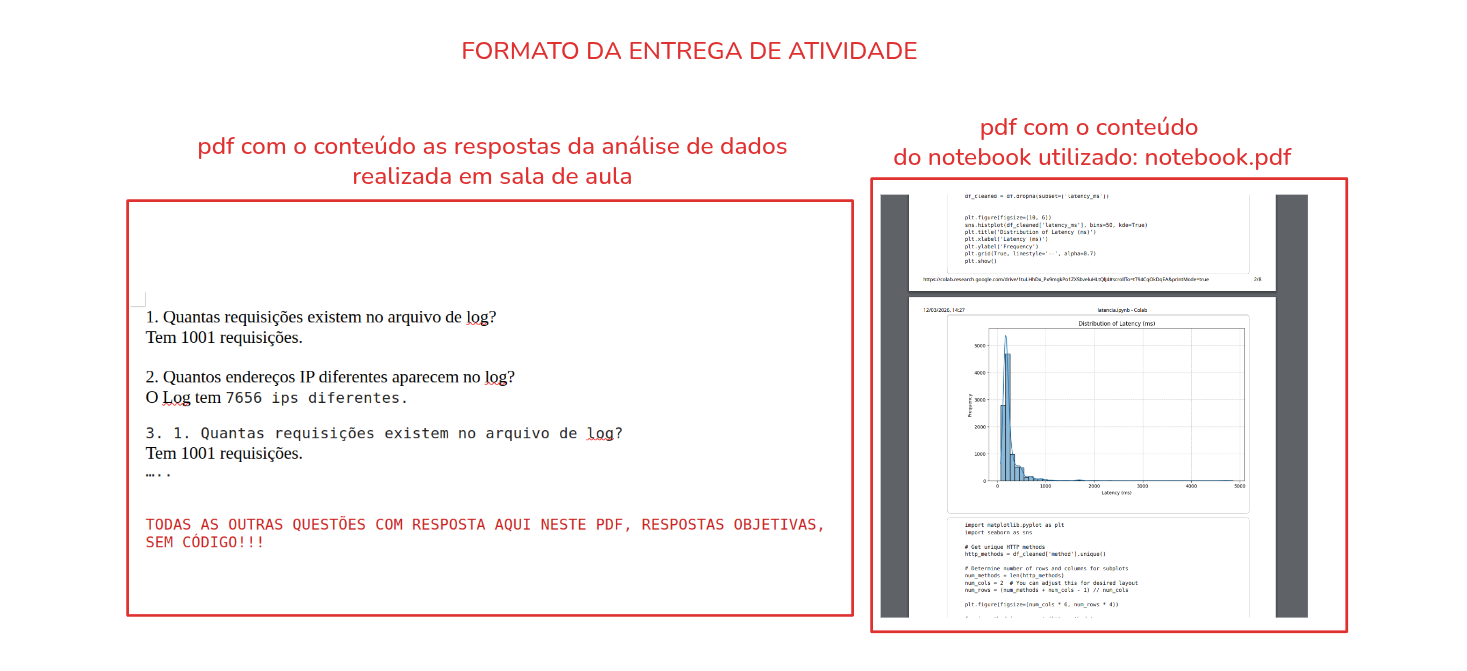
\includegraphics[width=\textwidth]{formato.png}
    \end{center}

\begin{block}{Parte 1 — Estrutura dos dados}

Responda:

\begin{enumerate}
\item Quantas requisições existem no arquivo de log?
\item Quantos endereços IP diferentes aparecem no log?
\item Quais métodos HTTP aparecem no conjunto de dados?
\item Qual o código de status mais frequente?
\end{enumerate}

\vspace{2cm}

\end{block}

\begin{block}{Parte 2 — Análise de latência}

Utilizando gráficos de distribuição:

\begin{enumerate}
\item Construa um histograma da latência das requisições.
\item Analise se a distribuição é simétrica ou assimétrica.
\item Existem requisições com latência muito elevada?
\item Qual é o percentil 90 da latência?
\end{enumerate}

\vspace{3cm}

\end{block}

\begin{block}{Parte 3 — Métodos HTTP}

\begin{enumerate}
\item Compare a distribuição de latência entre os métodos HTTP.
\item Algum método apresenta maior latência média?
\item Qual método apresenta maior variabilidade?
\end{enumerate}

\vspace{3cm}

\end{block}

\begin{block}{Parte 4 — Análise de erros e Confiabilidade}

Considere os códigos de status HTTP entre 400 e 599 como erros.

\begin{enumerate}
\item Quantas requisições resultaram em erro?
\item Calcule a \textbf{Taxa de Erro (Error Rate)} utilizando a fórmula:
\[ \text{Error Rate} = \frac{\text{Total de Erros}}{\text{Total de Requisições}} \times 100 \]
\item Calcule a \textbf{Disponibilidade (Availability)} do serviço:
\[ \text{Availability} = \frac{\text{Requisições com Sucesso}}{\text{Total de Requisições}} \times 100 \]
\item Compare a latência das requisições com erro e das requisições bem-sucedidas. O servidor demora mais para responder erros ou sucessos?
\end{enumerate}

\vspace{1cm}

\end{block}

\begin{block}{Parte 5 — SRE e SLAs (Service Level Agreements)}

A disponibilidade é frequentemente medida em "noves". Com base na tabela abaixo, em qual nível de disponibilidade o servidor se encontra?

\begin{center}
\begin{tabular}{|l|l|}
\hline
\textbf{Disponibilidade} & \textbf{Tempo fora do ar (por mês)} \\ \hline
99\% & $\sim$7h \\ \hline
99,9\% & $\sim$43 min \\ \hline
99,99\% & $\sim$4 min \\ \hline
99,999\% & $\sim$26 s \\ \hline
\end{tabular}
\end{center}

\begin{enumerate}
\item Se o acordo de nível de serviço (SLA) exigisse 99,9\% de disponibilidade, este servidor estaria cumprindo a meta?
\end{enumerate}

\end{block}

\begin{block}{Parte 6 — Requisições lentas}

Utilizando o percentil 90 de latência:

\begin{enumerate}
\item Identifique requisições com latência acima do percentil 90.
\item Quais URLs aparecem com maior frequência nessas requisições?
\item Existem IPs específicos associados a alta latência?
\end{enumerate}

\vspace{1cm}

\end{block}

\section*{Discussão}

Com base nas análises realizadas, responda:

\begin{itemize}
\item O servidor apresenta sinais de sobrecarga?
\item Existem indícios de acesso automatizado (bots)?
\item Quais possíveis melhorias poderiam ser aplicadas para reduzir a latência?
\end{itemize}

\vspace{4cm}

% =========================
\end{document}
% =========================